\documentclass{article}
\usepackage{graphicx} % Required for inserting images
\usepackage{amsmath}
\usepackage{amsfonts}
\usepackage{comment}
%\usepackage[backend=biber,style=alphabetic,sorting=ynt]{biblatex}  

\title{Blank project}
\author{Simon Eiriksson}
\date{October 2024}
%\addbibresource{references.bib}

\begin{document}
\section{Resume from meeting sept 27}
We aim to estimate the posterior predictive distribution of a new output $y^\ast$ given some input $x^\ast$
and given some previous data set $\underline y \vert \underline x$. This problem is phrased as

$$
p(y^\ast\vert x^\ast) = \int p(y^\ast\vert x^\ast, \theta)\cdot p(\theta\vert \underline y, \underline x)d\theta
$$

Here $p(\theta\vert \underline y, \underline x)$ is the posterior distribution over the weights, given the previously seen data. The problem here is that in general this integral is not analytically solvable, and so there is no exact solution to this problem. There are many ways to approximate the integral, most centred around sampling from $p(\theta\vert \underline y, \underline x)$. 

This can however be very computationally expensive, especially when $\theta$ is high-dimensional. One way to make such sampling more feasible is to use some approximation of $p(\theta\vert \underline y, \underline x)$.

\subsection*{Laplace approximation}

Laplace approximation is one such approach and takes the following direction.

Given some MAP-solution $\theta_0$ to the problem of maximizing the data log-likelihood $p(\underline y\vert \underline x, \theta)$, there exists a Gaussian distribution $q(\theta) \sim \mathcal N(\theta_0, \Sigma_0)$ with mean $\theta_0$, and similar hessian $H p(\underline y\vert \underline x, \theta) = H p(\theta_0)$. 

\subsection*{Riemann Laplace Approximation}

This is not necessarily a good approximation, if the data-likelihood is not “normal-shaped” around the MAP-solution. This can for example be the case if the weight posterior distribution is “banana-shaped” as seen in the figure. 
\begin{figure}[h]
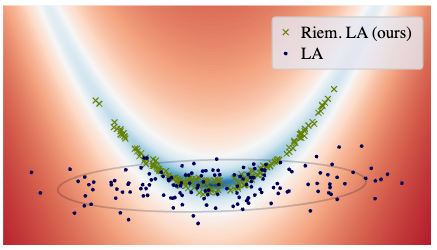
\includegraphics[width=0.5\textwidth]{banana.png}
\end{figure}


With Riemann Laplace Approximation, we use the Exponential mapping from Differential Geometry. The loss landscape induces a metric on the loss landscape manifold. This metric gives rise to shortest paths between points, as well as “shooting” trajectories: If a ball moves at constant speed from a point in some direction where will it be after some duration of time? In euclidian geometrics, the ball would follow a straight line, whereas in a non-euclidian geometric, this line would be curved. The point where the ball would be after 1 time unit, after being set in motion in direction $v$ from starting point $\theta$, is denoted $\mathrm{Exp_\theta(v)}$.

Now, rather than sampling from the Laplace approximation, we can sample from a normal distribution $v \sim \mathcal N(0, \Sigma_v)$, and then get $\theta = \mathrm{Exp}_\theta(v)$. 

This is basically what the paper “Riemannian Laplace approximations for Bayesian neural networks” does.

This is however highly computationally expensive (to calculate $\mathrm{Exp}_\theta(v)$), and if the parameter space is bigger than a few dimensions, we get into some of the same issues with curse of dimensionality as with MCMC sampling.

\subsection*{Task 1: Sampling from subspace Riemmannian data manifold}

What if we only sample from subspace spanned by the first $n$ eigenvectors of $\Sigma_v$? In that way we can reduce the dimensionality of the parameter space

\subsection*{Bayesian Quadrature}

Since for each sample of a direction-length $v$, the corresponding parameter $\theta = \mathrm{Exp}_\theta(v)$ is rather expensive to calculate, we can try to use Bayesian Quadrature to estimate the integral

$$
p(y^\ast\vert x^\ast) = \int p(y^\ast\vert x^\ast, \theta)\cdot p(\theta\vert \underline y, \underline x)d\theta
$$

using fewer samples, than we would if we just sampled the direction-length $v$ randomly from  $\mathcal N(0, \Sigma_v)$.

In general, Bayesian Quadrature aims approximate an integral over a probability distribution such as $\int f(v) \cdot p(v) dv$, by approximating $f$ by a Gaussian Process. The point here is that (if the kernel is gaussian????) the integral is then relatively cheap to calculate, including stochasticity.
\begin{figure}[h]
    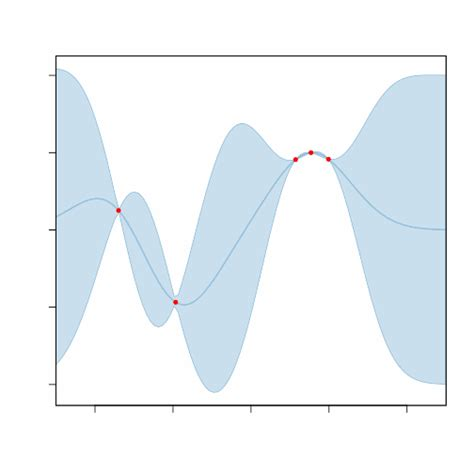
\includegraphics[width=0.5\textwidth]{GP.png}
\end{figure}
    

When generating the Gaussian Process, we can then sample values of $v$, where the variance is large, and where the prior probability $p(v)$ is high. In that way, we can reduce the variance of the integral approximation in the most efficient way.

This approach does however also only work in small dimensions (why??), which is why we will do the subspace sampling as in task 1 above.

\subsection*{Task 2: Bayesian Quadrature on subspace Riemmannian data manifold}

Let us try to do Bayesian Quadrature on the subspace given in task 1.

\end{document} 

